%
%
\documentclass[11pt]{scrartcl}

% own geometry
%\usepackage[a4paper, left=3cm, right=3cm]{geometry}

\usepackage[ngerman]{babel} 
\usepackage[utf8]{inputenc} 
\usepackage[T1]{fontenc}
\usepackage{graphicx}
\usepackage{color}
\usepackage{xcolor}
\usepackage{jurabib}
\usepackage{hyperref}

\renewcommand*{\jbauthorfont}{\textsc}
\renewcommand*{\bibfnfont}{\normalfont}
\renewcommand*{\biblnfont}{\textsc}
%\renewcommand*{\samepageibidemname}{Ebd.}
\renewcommand*{\bibbtsep}{In: }
\renewcommand*{\bibjtsep}{In: }
\renewcommand*{\bibpldelim}{(}
\renewcommand*{\biburlprefix}{}
\renewcommand*{\biburlsuffix}{}

\makeatletter
\renewcommand*{\jbshorttitlefont}{%
\ifthenelse{%
\equal{\jb@@type}{article}%
\or
\equal{\jb@@type}{periodical}%
\or
\equal{\jb@@type}{incollection}%
}{%
\upshape%
}{%
\textit%
}%
}
\makeatother

\renewcommand*{\bibprdelim}{)}
\renewcommand*{\ajtsep}{}
\renewcommand*{\bpubaddr} { :}
\renewcommand*{\jbbtasep} { ; }
\renewcommand*{\jbbfsasep} { ; }
\renewcommand*{\jbbstasep} { ; }
\renewcommand*{\bibbtasep} { ; }
\renewcommand*{\bibbfsasep} { ; }
\renewcommand*{\bibbstasep} { ; } %between second and third author sep
\renewcommand*{\jbbtesep} { ; } %between two editors sep
\renewcommand*{\jbbfsesep} { ; } %between first and second editor sep
\renewcommand*{\jbbstesep} { ; } %between second and third editor sep
\renewcommand*{\bibbtesep} { ; } %between two editors sep
\renewcommand*{\bibbfsesep} { ; } %between first and second editor sep
\renewcommand*{\bibbstesep} { ; } %between second and third editor sep
\AddTo\bibsgerman{\def\editorsname{(Hrsg.)}}
\AddTo\bibsgerman{\def\editorname{(Hrsg.)}}
%\jurabibsetup{super, citefull=first,ibidem}
%\jurabibsetup{ibidem}
%\jurabibsetup{authorformat=citationreversed}
%\jurabibsetup{authorformat=reducedifibidem}
\jurabibsetup{biblikecite}
%\jurabibsetup{bibformat=ibidem}
%\jurabibsetup{pages=always}
\jbfirstcitepageranges
\AddTo\bibsgerman{\def\herename{hier}}
\jbuseidemhrule

\jurabibsetup{
  authorformat={smallcaps,year,and,citationreversed},
  titleformat={colonsep,all,italic},
  commabeforerest,
  see,
  dotafter=bibentry,
  ibidem=strict,
  biblikecite
}

\renewcommand*{\bibbtasep}{ und } %
\renewcommand*{\bibbfsasep}{, }   %
\renewcommand*{\bibbstasep}{ und }
\renewcommand*{\jbtitlefont}{}
\renewcommand*{\bibtfont}{}
\renewcommand*{\bibbtfont}{}
\renewcommand*{\bibjtfont}{}
\renewcommand*{\bibapifont}{}
\renewcommand*{\jbshorttitlefont}{}



	%
	% CITATIONS
	%
\newcommand{\book}[2]{\footnote{\cite[Vgl.][#2]{#1}}}
\newcommand{\bookwf}[2]{\cite[Vgl.][#2]{#1}}
\newcommand{\bookdir}[2]{\footnote{\cite[][#2]{#1}}}
\newcommand{\inetwf}[1]{\cite[Vgl.][\citefield{url}{#1}]{#1}}
\newcommand{\inetwfdir}[1]{\cite[][\citefield{url}{#1}]{#1}}
\newcommand{\inet}[1]{\footnote{\inetwf{#1}}}
\newcommand{\inetdir}[1]{\footnote{\cite[][\citefield{url}{#1}]{#1}}}
\newcommand{\innerref}[1]{\footnote{Vgl. auch Kapitel \ref{#1} dieser Arbeit, S. \pageref{#1}}}
\newcommand{\vgl}[2]{\cite[Vgl.][#2]{#1}}
\newcommand{\citeauthoryear}[1]{\citeauthor{#1} (\citeyear{#1})}
\bibliographystyle{jurabib}

% setup of source code listings
\usepackage{listings}
%\usepackage{courier}
\usepackage{caption}
\lstset{
	basicstyle=\footnotesize\ttfamily,	% default font
	numbers=left,						% line numbers placement
	numberstyle=\tiny,					% line numbers style
	%stepnumber=2,						% line number padding
	numbersep=5pt,						% padding between line numbers and code
	tabsize=2,							% 
	extendedchars=true,         
	breaklines=true,						% line breaks 
	keywordstyle=\color{red},
	frame=b,
	stringstyle=\color{gray}\ttfamily,	% color of strings in code
	showspaces=false,					% visualize spaces
    showtabs=false,						% visualize tabs
    xleftmargin=17pt,
	framexleftmargin=17pt,
	framexrightmargin=5pt,
	framexbottommargin=4pt,
	showstringspaces=false				% visualize spaces in strings        
 }
 
 \lstloadlanguages{% Check docs for further languages ...
         C,
         C++,
         bash,
         HTML,
         Clean % use this for CSS
 }

\setlength{\parindent}{0pt}
\setlength{\parskip}\medskipamount

\DeclareCaptionFont{white}{\color{white}}
\DeclareCaptionFormat{listing}{\colorbox{gray}{\parbox{\textwidth}{#1#2#3}}}
\captionsetup[lstlisting]{format=listing,labelfont=white,textfont=white}

% layout the caption ontop of code
\captionsetup[lstlisting]{format=listing,labelfont=white,textfont=white, singlelinecheck=false, margin=0pt, font={bf,footnotesize}}

% Headings
\usepackage{fancyhdr}
\renewcommand{\footrulewidth}{0.4pt}
\cfoot{}
\rfoot{\thepage}

% Document begins now
\begin{document}

\author{%
	Oliver Erxleben \small(\href{mailto:oliver.erxleben@hs-osnabrueck.de}{oliver.erxleben@hs-osnabrueck.de})\\%
	Sergej Hert \small(\href{mailto:sergej.hert@hs-osnabrueck.de}{sergej.hert@hs-osnabrueck.de})\\%
	Jörn Voßgröne \small(\href{mailto:joern.vossgroene@hs-osnabrueck.de}{joern.vossgroene@hs-osnabrueck.de})\\
	\\%
	Hochschule Osnabr"uck \\%
	Ingenieurswissenschaften und Informatik \\%
	Informatik - Mobile und Verteilte Anwendungen\\
	Compilerbau - Sommersemester 2013 }

\title{
\includegraphics[scale=0.75,keepaspectratio]{img/hs_os.png}\linebreak \linebreak Implementierung eines Source-To-Source-Compilers zur Optimierung von CSS-Dateien im Webstack}

\maketitle
\thispagestyle{empty}
\pagebreak
\thispagestyle{empty}
\tableofcontents

\listoffigures

\lstlistoflistings
\thispagestyle{empty}
\pagebreak
% TODO: mehrseitiges Inhaltsverzeichnis ohne page numbering
\thispagestyle{empty}

\begin{abstract}

% TODO: überarbeiten
\textbf{Zusammenfassung:}\\ 	
Die vorliegende Ausarbeitung wurde in LaTex verfasst und ist eine gemeinsame Arbeit von Oliver Erxleben, Sergej Hert und Jörn Voßgröne an der Hochschule Osnabrück / University of Applied Sciences im Fachbereich Ingenieurswissenschaften und Informatik für das Fach Compilerbau im Sommersemester 2013. Die Arbeit beschäftigt sich mit der Optimierung von Cascading Stylesheets für Webseiten.\\
\\
Die Arbeit gliedert sich in mehrere Abschnitte. Im ersten Kapitel wird der Hintergrund des Themas beschrieben und es werden wichtige Fachbegriffe definiert. Ausserdem werden die Anforderungen an die Software aufgestellt.\\
Im zweiten Teil, Cascading Style Sheets, werden die Sprache, dessen Verwendung, sowie die zugrundeliegende Grammatik erläutert und es wird beschrieben wie Webbrowser diese interpretieren.\\
Der dritte Teil erläutert das Vorgehen der Optimierung. Neben der Syntaxanalyse und dem Optimieren der Knoten, wird auch die Implementierung eines Kommandozeilenwerkzeugs zur Steuerung der Optimierungen erläutert.\\
Der Abschnitt Messungen erklärt das Vorgehen für Tests. \\ Im abschließenden Abschnitt wird die Arbeit resümiert, das Ergebnis zusammengefasst und gewonnene Erfahrungen geschildert.   
\end{abstract}

\pagebreak
% set new page style

\pagestyle{fancy}
\setcounter{page}{1} 

% Einleitung 
\section{Einleitung}

\subsection{Motivation}
Im Alltag eines Frontend-Entwicklers, eines Mitarbeiters an einem Web-Projekt oder des Entwicklers für das grafische User Interface kommt es nicht selten vor, dass die Beschreibung der grafischen Elemente durch Cascading Stylesheets geschieht. Noch seltener sind diese Style Angaben fehlerfrei. Sei es aufgrund von Zeitdruck, unterschiedlichen Entwicklern oder durch nachträgliches Bugfixing, oft sind CSS-Regeln inkonstistent aufgestellt, zum Beispieln existieren noch Regeln, die garnicht mehr im DOM der Seite zu finden sind. Es werden Regeln mehrmals überschrieben und es wird nicht auf Optimierung von Selektoren geachtet. 

Seit 2010 berücksichtigt der Page Ranking Algorithmus von Google auch die Ladezeiten für Websites\footnote{Offizieller Blogpost von Google: http://googlewebmastercentral.blogspot.de/2010/04/using-site-speed-in-web-search-ranking.html}. Seiten, die neben SEO\footnote{SEO: Search Engine Optimization / Suchmaschinenoptimierung} ein gutes Page Ranking erhalten, werden demnach auch durch ihre Ladezeiten bestimmt. Die Ladezeiten spielen zwar im Vergleich mit SEO nur eine kleine Rolle, können aber zu einem besseren Ergebnis beitragen (Weite Informationen: http://googlewebmastercentral.blogspot.de/2010/04/using-site-speed-in-web-search-ranking.html).
Ladezeiten von mobilen Websites und Web-Anwendungen bzw. Seiten, die über mobile Internetverbindungen geladen werden, sollten schnell und nur wenig Daten übertragen, um ein konsistentes Benutzererlebnis zu gewährleisten. Statistiken zeigen, dass Benutzer auf Websites eher verbleiben wenn diese schnell geladen werden und der Benutzer schnell Informationen abrufen oder mit der Anwendung interagieren kann.

\subsection{Anforderungen}

Im Rahmen der Hausarbeit für das Fach Compilerbau im Sommersemester 2013 im Master-Studiengang Informatik - Verteilte und Mobile Anwendungen an der Hochschule Osnabrück / University of Applied Sciences soll ein Werkzeug entwickelt werden mit dem sich Stylesheets optimieren lassen. Das Parsen der CSS-Quellen soll mittels Flex und Yacc, bzw. Bison geschehen. Vgl. siehe \cite{appel_cc}.

Weiterhin soll ein Kommandozeilentool entwickelt werden, womit CSS-Optimierungen gesteuert und ausgegeben werden können. 

Nachfolgend werden die Anforderungen beschrieben.

\begin{description}
    \item[Ausgabeformat] Das Ausgabeformat soll ebenfalls als CSS-Datei geschrieben werden.
    
    \item[Ungenutztes CSS entfernen] Deklarierte Regeln die in HTML-Dateien nicht eingesetzt werden, sollen entfernt werden, da sie überflüssig sind.
    
    \item[Gleiche CSS-Regeln zusammenführen] Selektoren die mehrmals in den CSS-Dateien vorkommen, werden zu einer Datei zusammengeführt, wobei bei gleichen Eigenschaften der neuere den älteren Wert überschreibt (Kaskade).
    
    \item[Shorthands für Hex-Farbwerte] Manche Farbewerte lassen sich verkürzt darstellen. So erzeugt der Hex-Farbwert \textbf{\#fff} ein gleiches Ergebis wie der (längere) Wert \textbf{\#ffffff}. 
    
    \item[]
\end{description}

Die vorgestellten Anforderungen an den CSS-Optimierer werden in der Abbildung \ref{app-workflow} als Flow-Diagram beschrieben. 

\begin{figure}[h!]
	\begin{center}
		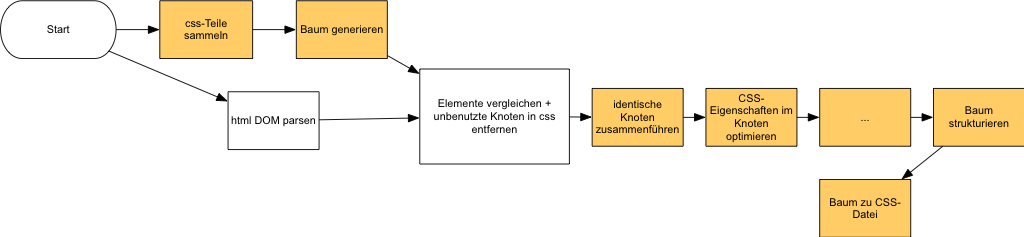
\includegraphics[width=1.0\textwidth]{img/app-workflow.png}
		\caption{Workflow der Anwendung}
		\label{app-workflow}	
	\end{center}
\end{figure}
\pagebreak

% Einführung in CSS
\section{Einführung in CSS}
\subsection{Cascading Stylesheets}

Cascading Stylesheets gilt aktuell als Standard-Stylesheetsprache für Websites. Es findet aber auch Verwendung in anderen Umgebungen, wie zum Beispiel JavaFX. Mit CSS ist es möglich Ausgabemedien unterschiedliche Darstellung vorzugeben. Beispielsweise soll einen Hyperlink\footnote{Hyperlink:} beim Druck einer Seite in einer anderen Farbe dargestellt werden oder die Elemente einer Bildergalerie sollen auf Geräten mit kleinerer Auflösung (wie etwa Tablets oder Smartphones) gelistet werden und bei einem Display mit FullHD-Auflösung können Bilder in einem Gitternetz dargestellt werden. 

Verschiedene spezielle CSS-Eigenschaften können für die unterschiedlichen Einsatzgebiete von CSS existieren. Die vorliegende Ausarbeitung bezieht sich auf CSS im Web-Stack, bzw. untersucht nur CSS für Webseiten. 

\subsection{Revisionen und Probleme}
Die Entwicklung von CSS wurde 1993 begonnen und hat nach mehreren Versionen 1995 den Stand der ersten Version erreicht. 1998 wurde die Version zwei vorgestellt. Diese ist aktuell und wurde bis heute allerdings von keinem der Mainstream-Browser vollständig implementiert. Einige Browser setzen große Teile des CSS2, bzw. CSS2.1-Standards korrekt um. Es kann aber zu Problemen bei unterschiedlichen Browsern führen. 2011 wurde die Recommandation für CSS 2.1 veröffentlicht. 

Die aktuelle Entwicklung für den dritten Standard von CSS begann bereits 2000. Zu den Neuerungen in dieser Revision gehören vor allem der modulare Aufbau, womit CSS-Eigenschaften nun schrittweise entwickelt werden können. Fast alle Browser implementieren Kernfunktionen des dritten CSS-Standards, die allerdings variieren können. 

\subsection{Allgemeiner Aufbau}

Damit eine Optimierung von bestehenden CSS-Quelltext durchgeführt werden kann, muss zuvor analysiert werden wie ein Browser CSS verarbeitet und wie Kaskadierung im Browser genutzt wird um Style-Informationen zu verknüpfen.

Eine CSS-Datei besteht aus einer Menge von Anweisungen, oder Regeln, die das Layout einzelner Elemente (mit bestimmter ID), Klassen von Elementen oder allgemein gültigen Elementen bestimmen. Regeln deren anzuwendenen Eigenschaften gleich sind, können mittels Kommata getrennt werden. Es ist zudem möglich

% TODO: Tabelle vom w3c

Der allgemeine Aufbau einer CSS-Regel wird im Listing \ref{css_basics} veranschaulicht.   
%TODO comment in css style
\begin{lstlisting}[label=css_basics,language=bash, caption=Aufbau einer CSS-Regel]
a {
    background:#000;
    color: #fff;
}  
#special {
    border: 1px solid red;
}

.left, top.myClass {
    border: 1px dotted green;
}
\end{lstlisting}

Im Listing sind drei Regeln gegeben. Die erste Regel wird für ein HTML-Element angewendet. Jedes a-Element (Links im Browser) werden schwarz unterlegt und der textliche Inhalt des Elements wird weiß dargstellt. Bei dem zweiten Element wird eine Regel auf ein Element mit der ID \textbf{special} angwendet. Dies erhält einen durchgehenden roten Rahmen um den Inhalt des Elements. Die dritte Regeln legt eine gepunktete grüne Linie um den Inhalt der Elemente mit der Klasse \textbf{left}, sowie der HTML-Elemente top mit der zugewiesen Klasse \textbf{myClass}.  

Wie interpretiert der Browser allerdings die vordefinierten Werte mit den kaskadierten Elementen der Stylesheet-Datei und wie berechnet sich daraus der zusammengesetzte Wert? Dazu sei die Abbildung [] gegeben. %TODO: Abbildung für CSS-Berechnung im Browser 

% TODO: Table
\subsection{Syntax}
% TODO: Syntax W3C

% TODO: Tabelle Selektoren

\subsection{Grammatik}
Die zugrundeliegende Grammatik stammt von der Seite des W3C (Details, siehe: \cite{w3c_css_grammar}). Dies entspricht im Wesentlichen der Grammatik für die CSS Version 2.1. Das Listing \ref{css_grammar} zeigt die Grammatik des W3C. 

Für die Optimierung einer CSS-Datei ist diese Grammatik allerdings ungeeignet. Zum einen gehört die Grammatik zu einer älteren CSS-Version und zum anderen ist die Aufgabe des Optimierers nicht die Darstellung oder die Interpretation der CSS-Quelldateien, sondern die Verbesserung der definierten Elemente nach definierten Regeln. Dafür wurde eine eigene Grammatik entwickelt. Diese wird im Abschnitt \ref{tree_generation_used_grammar} vorgestellt. 



\pagebreak

% Kommandozeilenwerkezeug
\section{Kommandozeilenwerkzeug}
Um Optimierungen durchzuführen wurde im Rahmen der Hausarbeit ein Kommandozeilenwerkeug erstellt, welches in den folgenden Teilabschnitten vorgestellt wird.

\subsection{Makefile und Start des Programms}
Zur Kompilierung und Bereitstellung wurde ein Makefile erstellt (Details siehe Listing \ref{makefile_listing}). Mit dem Makefile besteht ebenfalls die Möglichkeit Einzelteile des Projekts zu erstellen. Zum Beispiel kann mittels \textbf{make parser} nur der Parser erstellt werden.

\begin{lstlisting}[label=makefile_listing,language=C, caption=Makefile]
#include grammar/makefile.mk

all: app
	
app: lex.yy.c test.tab.c test.tab.h grammar/css_types.h
	cc grammar/test.tab.c grammar/lex.yy.c grammar/css_types.c main.c cli_parse.c css_merge.c guiCSS.c optimizer.c output.c -lncurses -o optimCSS
	
parser: lex.yy.c test.tab.c test.tab.h grammar/css_types.h
	cc grammar/test.tab.c grammar/css_types.c grammar/lex.yy.c -o parser

test.tab.c test.tab.h: grammar/test.y
	bison -d grammar/test.y -o grammar/test.tab.c
            
lex.yy.c: grammar/test.l test.tab.h
	flex -o grammar/lex.yy.c grammar/test.l

clean: 
	rm -f lex.yy.c grammar/test.tab.h grammar/test.tab.c grammar/parser optimCSS
\end{lstlisting}

Der Start des Programms geschieht über die Konsole unter Angabe von Parametern. Zur Verfügung stehen die folgenden Parameter:

\begin{description}
   \item[ -f dateiname] Angabe der Quelldatei. Dies muss eine HTML-Datei sein. Aus der angegebenen HTML-Datei werden die genutzten CSS-Dateien extrahiert und zusammengeführt für die Optimierung.
   \item[ -m] Minifizierte Ausgabe.
   \item[ -s] Strukturierte Ausgabe.
\end{description}

Zum Start des Programms ist der Parameter -f zwingend nötig um dem Optimierer CSS-Dateien zur Verfügung zu stellen. Ein Beispiel ist in Listing \ref{example_program_start} dargestetllt.

\begin{lstlisting}[label=example_program_start,language=Bash, caption=Programmstart]

./optimCSS -f index.html

\end{lstlisting}

\subsection{Datenstrukturen}

Zum Einlesen der Kommandozeilen parameter und der HTML- bzw. CSS-Dateien wurden Datenstrukturen definiert. Diese sind in Listing \ref{datastructures_input_listing} dargestellt.
Mit Hilfe der Strukturen ist es möglich den Ausgabetyp, Eingabetyp, Eingabedatei sowie eine temporäre gemergte CSS-Datei zu halten.

\begin{lstlisting}[label=datastructures_input_listing,language=C, caption=Datenstrukturen]

enum output_type {STRUCTURED, MINIFIED};  // -s, -m
enum input_type {FILE_INPUT, PATH_INPUT}; // -f, -p

struct input_data {
	int output_type;
	int input_type;
	char* src;
};

struct css_data {
	char* src_html;
	char* merged_css;
};

\end{lstlisting}


\subsection{Grundaufbau des Kommandozeilenwerkzeugs}
Das Kommandozeilenwerkzeug lässt sich in fünf Komponenten unterteilen. In der ersten Komponente werden die Kommandozeilenparameter eingelesen und für die spätere Nutzung in einer Struktur abgelegt.
Die folgende Komponente ermittelt aus der übergebenen HTML-Datei alle genutzten CSS-Dateien und merged diese zu einer temporären CSS-Datei, welche später zur Optimierung verwendet wird.
Nachdem nun eine einzelne CSS-Datei zum Optimieren bereit steht wird diese zunächst mittel eines durch Flex und Bison erzeugten Parsers in eine Baumstruktur überführt und so für die eigentiche Optimierung aufbereitet.
Die hierzu genutzten Flex- und Bison-Quellen sind in den Listings \ref{css_lex} und \ref{css_bison} dargestellt. 
Auf dem nun vorliegenden CSS-Baum werden nachfolgend einige Optimierungen durchgeführt, welche in Kapitel \ref{chap_optimization} detaillierter beschrieben werden.
Abschließend wird der optimierte CSS-Baum in Textform als CSS-Datei ausgegeben. Die Ausgabe kann sowohl strukturiert (gut lesbar) als auch minifiziert erfolgen. Dies wird mittels Kommandozeilenparameter eingestellt.




\pagebreak

% Baumgenerierung
\section{Baumgenerierung}
\subsection{Aufbau,}
\subsection{Verwendete Grammatik}
\label{tree_generation_used_grammar}
% TODO: Listing eigene Grammatik
Der Baum soll nach
\subsection{Ausgabe}


\pagebreak

% Optimierung
\section{Optimierung}

\subsection{Syntaxanalyse}
\subsection{Knotenoptimierung}

\pagebreak

\section{Messungen und Ergebnis}
\subsection{Grundlage}
Als Grundlage zur Bewertung von Optimierungen, soll eine größere \textbf{Single Page Applikation} verwendet werden. Single Page Anwendungen folgen dem Paradigma niemals die gesamte Seite neu zu laden, sondern nur gewünschte Teile der Anwendung zu aktualisieren. Oft werden dabei asynchrone Requests oder auch Web-Sockets verwendet. Dies verbessert Ladezeiten, SEO, ... 
% TODO: überarbeiten, auf Korrektheit prüfen.



Weiterhin wurde ein eigener minimalistischer Webservice, basierend auf \textit{Ruby Rack} und \textit{WEBrick}, entwickelt. Der Webdienst dient zur Bereitstellung der Testdaten vor und nach der Optimierung. Das Listing \ref{server_rb} zeigt die Implementierung des Dienstes, welcher den aus der Standard-Ruby-Implementierung mitgelieferten Web-Server nutzt und auf Port 80 lauscht. 

\begin{lstlisting}[label=server_rb,language=Ruby, caption=Ruby Webservice für Messdaten]
#!/usr/bin/env ruby

# USAGE: ./server.rb path/to/the/root/dir

require 'rubygems'
require 'rack' # rack it up

serve = Rack::Builder.new do
 use Rack::Static, 
   :urls => ["/images", "/js", "/css"],
   :root => ARGV[0],
   :index => 'index.html'
 run Rack::File.new(ARGV[0])
end

# by default WEBrick doesen`t listen to sigkill, cause the script runs in a new session. 
Signal.trap('INT') {
  Rack::Handler::WEBrick.shutdown
}

# takeoff
Rack::Handler::WEBrick.run(serve, :port => 80, 'Contetn-Type'=>'text/html')
\end{lstlisting}
% TODO: Bibliotheken
\subsection{Bewertungskriterien}

\subsection{Ergebnisanalyse}

% TODO: Als Tabelle
\begin{table}[ht!]
	\centering
	\begin{tabular}{c | c}
		Anforderung & Beschreibung \\
		\hline
		Ausgabeformat & optimiertes CSS soll entstehen \\
		5 & Spieler ist weiß und beginnt \\
		6 & Spieler hat gewonnen \\
		7 & Spielfeld voll \\
		8 & Start einer neuen Runde \\
	\end{tabular}
	\caption{Anforderungen an die Optimierungen}
	\label{server-proto-bit-usage}
\end{table}
\pagebreak
\thispagestyle{empty}

\renewcommand*{\biburlprefix}{(URL: }
\renewcommand*{\biburlsuffix}{)}

\pagebreak
\addcontentsline{toc}{section}{Literaturverzeichnis} % Eintrag ins Inhaltsverzeichnis
\bibliography{bib/bib}

\appendix
\addcontentsline{toc}{section}{Anhänge}
\thispagestyle{empty}
\section*{Virtuelle Maschine}
Zur Messung der Testdaten wird eine virtuelle Maschine erstellt. Diese liegt dem Datenträger als VirtualBox-Maschine dieser Hausarbeit bei. 

\subsection*{Betriebssystem}
Als Betriebssystem dient ein aktuelles Debian Linux mit einem virtuellen Kern, 256 MB Arbeitsspeicher und 8 GB Massenspeicher. Diese Hardwarespezifikation entspricht im wesentlichen eingebetteten Systemen oder Shared Webhosting. 

\subsection*{Benutzer- und Logindaten}

Für die VM wurde folgende Benutzer mit Passwort angelegt:
\begin{itemize}
    \item{cbh:compiler (Standardbenutzer)}
    \item{root:r00t (Superuser)}
\end{itemize}

\subsection*{Dienste und Tools}

Auf der virtuellen Maschine sind folgende Dienste und Werkzeuge installiert: 

\begin{itemize}
    \item{FTP}
    \item{Ruby}
    \item{SSH}
    \item{Git}
\end{itemize}

Dem FTP- und SSH-Server ist der Standardbenutzer zugewiesen, sodass Dateien auf, bzw. von dem Server geladen werden können.

\subsection*{Ordnerstruktur}
Im Homeverzeichnes des Benutzers \textit{cbh} befindet sich das Git-Projekt \textit{compilerconstruction}.
% TODO: Beenden

\end{document}
